\section{Protecting Metadata}
Once a message has been received at the client, we would like to upload it to the IMAP server for storage. Yet while we can hide the FROM and TO headers easily, we do not want the server to gain timing information about the message. If we upload it immediately, then the server will know that we have received a message at that time. Even worse, modern clients often save sent messages to a Sent Messages folder. If the mail server of the sender and the receiver are colluding, as can easily be the case when both clients are using the same company to provide servers, then the server could easily execute timing attacks by observing two users suspecting to be communicating, and seeing if they upload a message at about the same time. So, we must include a mechanism for hiding this timing metadata from the IMAP server. The solution must not allow the server to recover the timing information, it must not take up extraneous amount of space in the mailbox, and it must allow sufficiently frequent and short exchanges with the server. Additionally, for any of these methods, the deletion of a message from the server must not reveal otherwise hidden information.

\subsection{Mechanisms}
While we can vary particular parameters and algorithms, most rely on two primary components, scheduling and mixing.

  \begin{tikzpicture}[node distance=8cm]
  \node (\project) [box, minimum height=2cm] {\project};

  \node (scheduler) [box, minimum height=2cm, right of=\project] {Scheduler};

  \draw [arrow] (\project.10) -- node [above] {State information} (scheduler.-190);
  \draw [arrow] (scheduler.190) -- node [below] {Next action type} (\project.-10);
 
  \end{tikzpicture}

Fundamentally, scheduling means that \project performs an action at a predetermined time tick. To better reason about the leakage of information, \project contains a separate scheduler module (shown above) that is informed when a message arrives or is marked for deletion. It thus can reason about the expansion rate of the server. At the scheduled time tick, \project will ask the scheduler what its next action should be. This can be one of three types: UP, DOWN, or NONE. UP means that the server will grow in size by one message, DOWN means that it will shrink by one message, and NONE means that the total server size will remain constant. The trit that it outputs is based on its metadata protection policy, determined in conjunction with the \project module. We separate this functionality into the scheduler because it precisely mirrors the information that the server will receive: whether a message has been pushed up, pulled down, or neither. Thus, the server can gain no more than one trit of data on every time tick.

To implement this one-trit leakage, \project must perform the determined action on each timer tick, whether or not it is has a message to deliver or a deletion scheduled. This condition is satisfied through artifically constructed messages. A constructed message with contents of a random size chosen from a distribution mirroring that of messages usually sent and received of the user is generated, encrypted and packaged as if it were a legitimate message, saved to a FAKE MESSAGES PSEUDO-mailbox, and sent to the server. On deletion, a message from FAKE MESSAGES is chosen at random and deleted in lieu of a legitimate message. Without taking into account any other information, these actions would appear identical to the server whether they were performed on real or fake messages, since the server will see only updates to the INDEX and the append or delete of a message with subject ENCRYPTED <UNIQUE SUBJECT> and encrypted contents. How they appear to the server in the context of all actions performed is the subject of Section~\ref{best-metadata}.

\project also incorporates mixing to better hide metadata. In a single mixing step, MIX NUMBER messages are fetched and deleted from the server, and MIX NUMBER $\pm 1$ messages are pushed back to the server so that a particular message in the former set can be associated with all messages in the latter set with equal probability. Note that for mixing to be effective, all messages included in the mix must be of the same size. Which messages are selected to be a part of the mix depends on the metadata hiding strategy.


\label{best-metadata}
\subsection{Strategies}

The requirements that \project has for operations on messages bear resemblance to those of memory operations in oblivious random access memory (ORAM)\cite{oram}. ORAM assumes a situation where multiple actors (say CPUs) can see memory access and store actions on a shared memory module. It proposes a system of additional memory accesses and locations to shield patterns of which memory locations have been accessed. ORAM techniques and implementations are an active area of research, some with proven lower bounds on additional bandwidth cost \cite{stefanov2013path}.

ORAM makes assumptions that we could perhaps consider relaxing. First, ORAM assumes constant, fixed-size blocks of memory. Messages in a mail server need not be constant size, although any solution that involves mixing will require elements of the mix to all be of the same size. Second, a primary goal of ORAM is to hide correlated memory locations. If messages are not decomposed into fixed-size chunks and all saved into the same pseudo-mailbox, then an individual message is not correlated with any other message. Note that mixing will generally require chunking of messages, and we wish to support multiple pseudo-folders, but locations are not as inherently correlated in all cases as they are when a program is executing on memory locations. Third, mailboxes do not allow store operations in the sense of RAM; IMAP only supports appending to mailboxes. Even under these relaxations, most solutions that do not implement an ORAM-adherent technique will trade off either functionality or security.

\subsubsection{Scheduling without mixing}
Could we implement a mix-free solution where we only schedule UP and DOWN operations, hiding actual message additions and deletions among many fake ones? In such a situation, future actions should not reveal information about which messages previously pushed were real and which were fake. Particularly, assuming that deletions of fake messages occur much more frequently than deletions of real messages, deletion operations should reveal neither whether the particular message deleted or any other was real. Additionally, message fetches must similarly not reveal information regarding the veracity of that message or any other. Note that this last restriction immediately disqualifies this solution barring additional mechanisms to mask message fetches by any client of the server that attempts to download all real messages. Further, naive fetches would leak information about which messages are grouped together in a single mailbox. We will see that it is not practical to attempt to find such mechanisms, since the rate of growth required to sufficiently mask deletion operations is infeasible.

Consider the trivially incorrect case where server growth roughly mirrors the rate of incoming real messages. We upload two messages to the server, R and F. R is a real message, and F a fake. Initially, the server cannot distinguish between the two messages. Since R is real, there is some user-dependent probability $p$ that it will be deleted at any point in the future. Given the availability of storage, a modern trend of archiving, and that these messages are encrypted, we can assume that $p$ is very small. Since we are looking to have server growth mirror the rate of incoming real messages, the goal of the scheduling algorithm is to send messages to the server at an effective rate similar to the rate of actual message receipt, so the server does not grow needlessly. Then, the number of fake messages will remain about constant, $k$. So at each timer tick where a DOWN occurs, a fake message will have probability $p=1/k$ of being deleted. Therefore, the probability that a message is not deleted after $n$ DOWN ticks is $(1-1/k)^n$ (since it must not be deleted at all time ticks), which tends towards 0 as $n$ increases. Thus, a fake message's long-term probability of being deleted is 1. So, after a length of time has passed, any message that was uploaded to the server and has remained there for a long period of time is likely a real message, and the server can therefore merely observe the time it was uploaded.

This analysis does not only apply in the theoretical sense. Assume the user had let the system run in a mode where more fake messages are uploaded than are deleted until it was seeded with 5,000 fake messages. After that point, the user wants to keep the size of the mailbox constant, so for each upload (received message), they delete a message as well. Assume also that they would like to spread new messages to other clients of the server within 10 minutes of its receipt (a conservative estimate). Then they must delete a message every 10 minutes as well, which amounts to 144 deletions a day, 52,560 a year, and 262,800 in a five year period, which we conservatively assume is the length of time a user would like to keep an email account for. So $k=5000$ and $n=262800$, giving a probability of a fake message not being deleted of about $1.5\times10^{-23}$, which is certainly distinguishable from $p \approx 1$ for a real message.

Now assume instead that we will let the server grow to some extent. By adding more fake messages than real messages, we will drive down the probability that a fake message is chosen for deletion until it resembles the probability that a real message is chosen. How often could we delete messages chosen from the set of all fake messages at random before we lose the ability to hide real messages among the fake ones? Assume for simplicity that fake messages are added at an amortized constant rate. We would like to calculate the probability that a fake message is not deleted after the $n$ DOWN ticks following its upload at time $t$. This is equal to the product of the probabilities that a fake message was not deleted at all ticks between times $t$ and $t+n$. We can compute this based on the probability of deleting a message at a particular time after $i$ deletion intervals. Assume that at each each interval, $c+1$ real messages and $f$ fake messages came in. Then the probability that a message was fake is $f/(c+f+1)$, and $c+f+1$ messages total came in each interval. But one message was deleted each interval, so $c+f$ net messages are added. So after $i$ intervals, $i(c+f)$ messages are in the server total, and an expected $i(c+f)f/(c+f+1)\approx if$ of those are fake. So the probability of a message being deleted at time $i$ given that it is fake is $1/(if)$, and the probability that it is not deleted is $1-1/(if)$. Then if the message was uploaded at time $t$, the probability that it was not deleted at time $n$ is $\displaystyle\prod_{i=t}^{i=t+n}(1-\frac{1}{if})$. This product tends towards 0 as $n$ tends towards infinity, but its slope drops off quickly as $f$ increases.

For example, consider the following graph of the probability of a message being not deleted from when it was added at time $i=250$, until time $i=1000$.

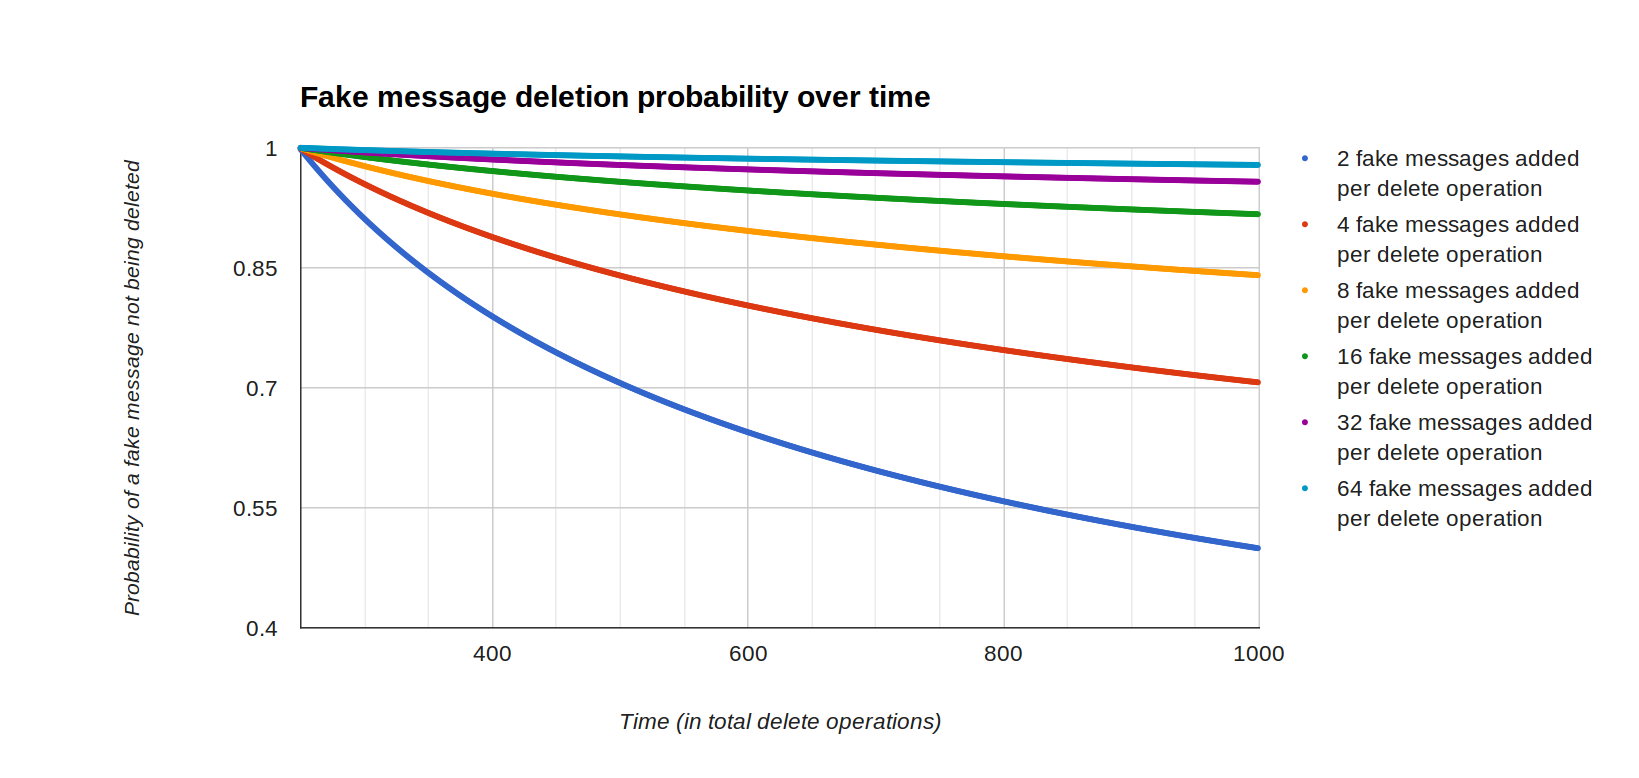
\includegraphics[width=\textwidth]{many_lines_2}

Note that if 32 or 64 messages are added per deletion operation, the probability that a fake message is not deleted remains at 0.96 and 0.98 even after $1000-250=750$ operations. This comparison is shown more clearly in the following graph.

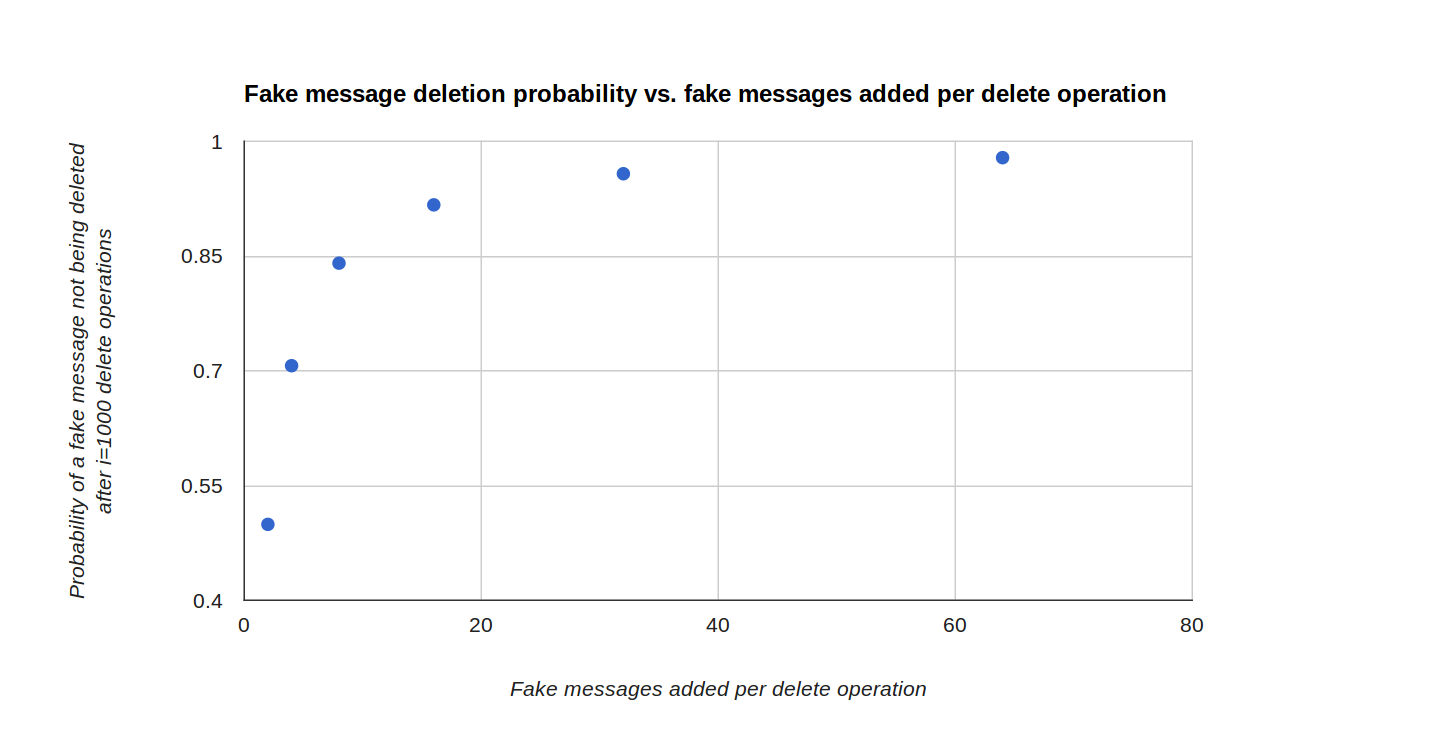
\includegraphics[width=\textwidth]{few-blue-dots-250}


Yet we only achieve these high rates after the server has been seeded with an adequate number of fake messages, as demonstrated by altering our parameters to show the results when a fake message is instead added at interval $i=0$.

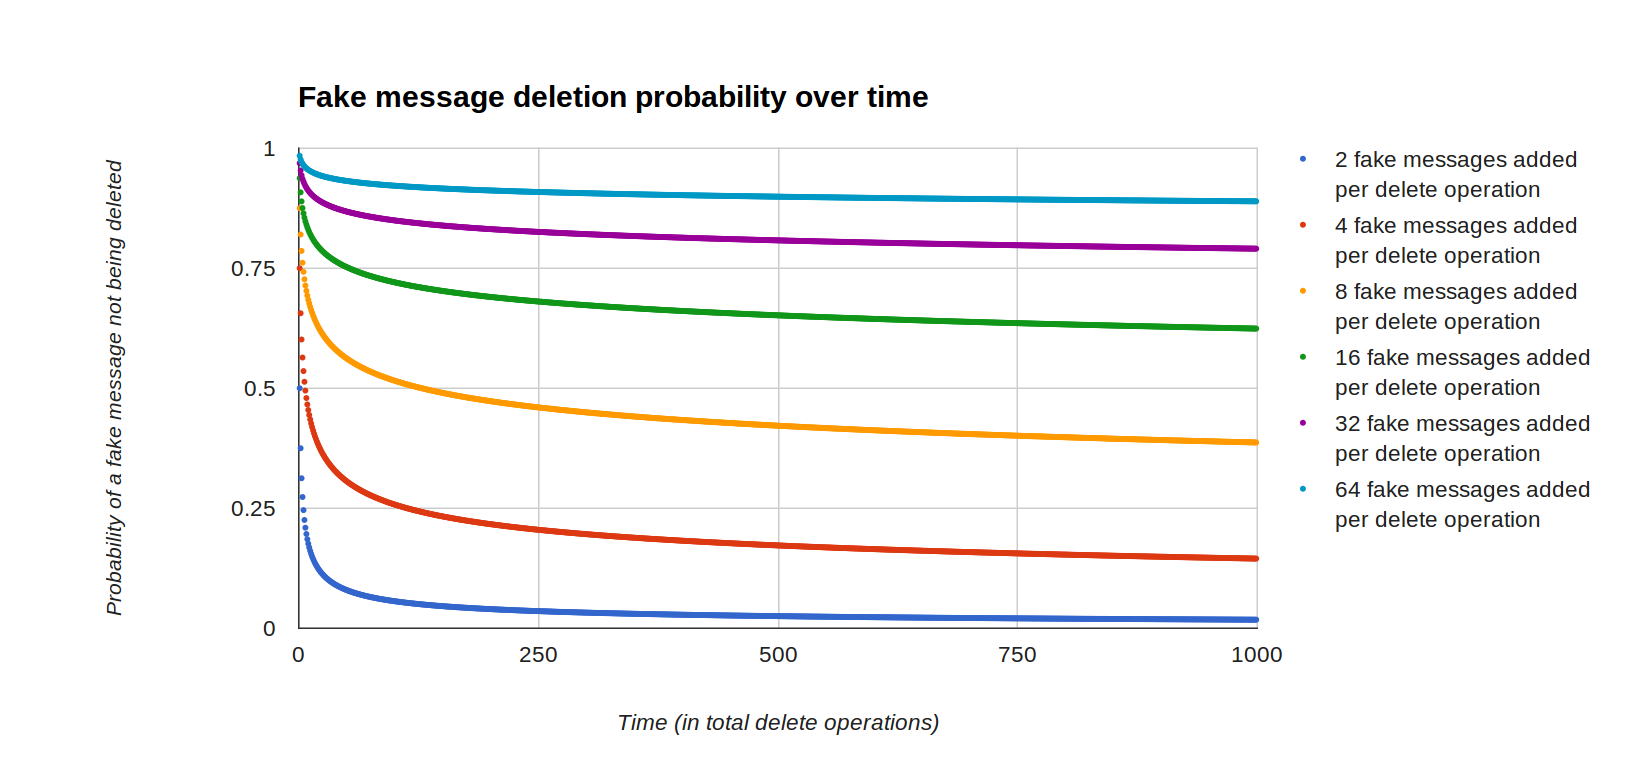
\includegraphics[width=\textwidth]{fake-message-deletion-over-time}

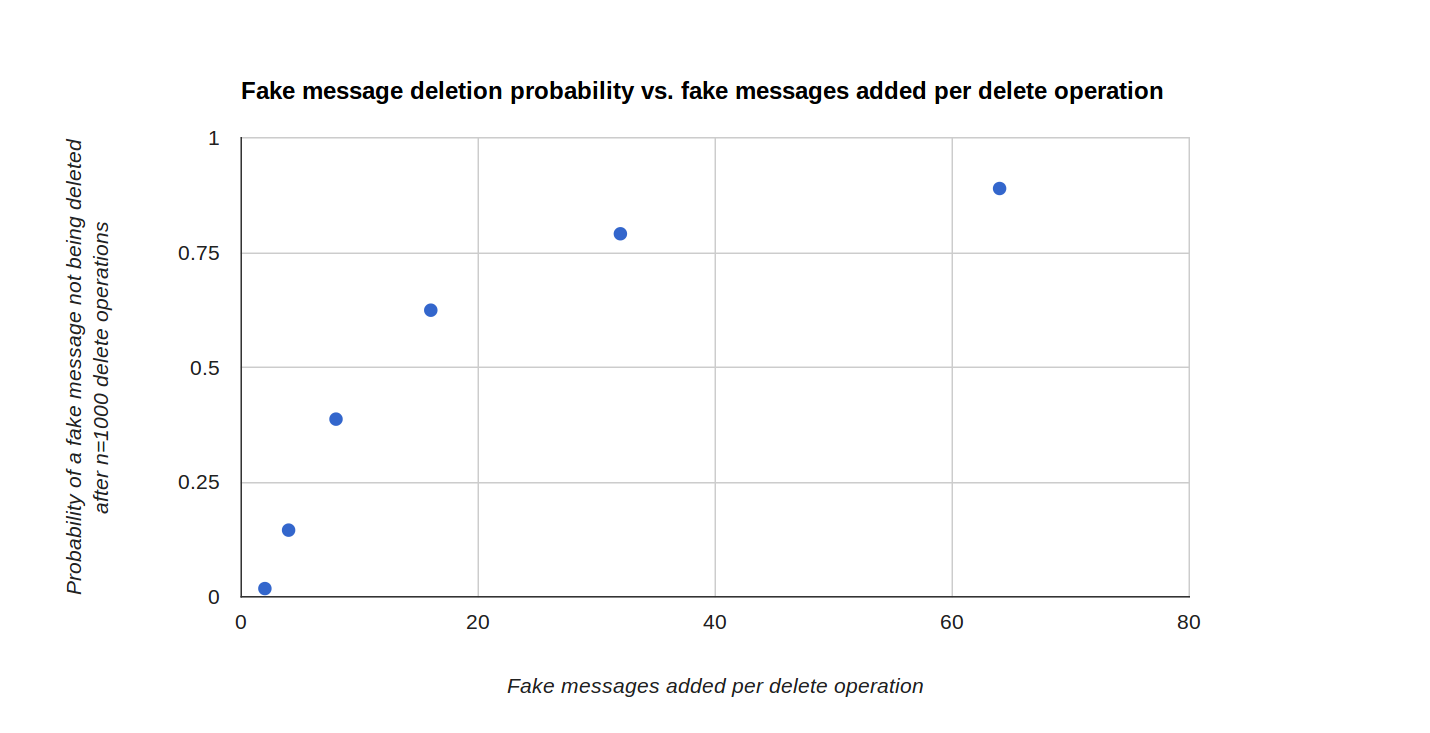
\includegraphics[width=\textwidth]{fake-message-deletion-probability-vs-num-fake-messages-added}

In this case, we need an $f$ of 64 to achieve merely a $p=0.89$ that a fake message is not deleted (compare, of course, with $p=1$ for a real message under the assumption that no real messages are ever deleted). Thus, to achieve even a relatively feasible probability match, we could delete only 1 in 64 messages.

Is this rate of growth sustainable? Theoretically it is, of course, but not given reasonable expectations of server longevity. Assume we would like to delete a message every 64 messages that were pushed, and that one operation occurs per time tick. The following graph relates message check frequency for varying numbers of clients connected to an IMAP server with time to fill a mailbox. The total mailbox size is Gmail's current size of 17 GB, and an average message is 170 kB.

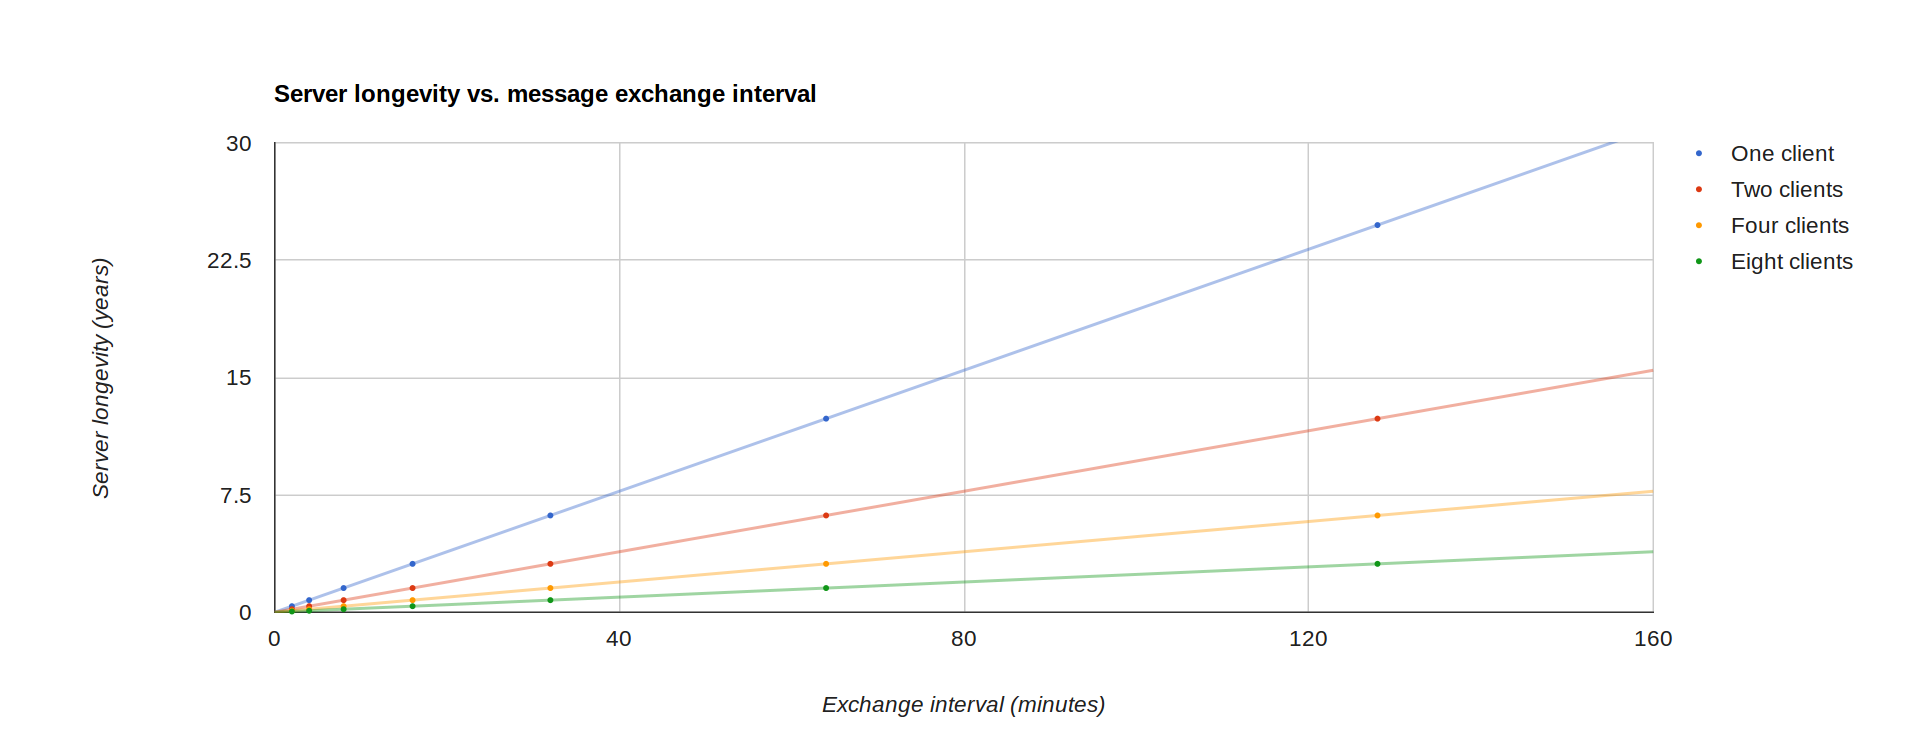
\includegraphics[width=\textwidth]{server_longevity}

With only two clients, if we wish to check our mail more than once every half hour (both of which are conservative estimates), we would use up the space in three years. To compensate for space costs with, we can introduce mixing operations.

\subsubsection{Mixing with \texorpdfstring{$O(1)$}{O(1)} decoys}

If we wish the growth rate of the server to precisely match the rate of messages to be pushed, we must perform many mixing operations. Intuitively, this is because to grow with the actual rate, each fake message that was in an UP operation must appear in a DOWN operation. Mathematically, assume that the mailbox is seeded with $k-1$ fake messages. Consider again messages R and F, and call MIX NUMBER $m$. This time, R and F were each one of $m + 1$ messages pushed to the server, with R pushed into set A and F pushed into set B. Assume no overlap between A and B, since $m<<n$, the total number of messages. This case is similar to the case of no extraneous growth without mixing assessed above, since we are extremely unlikely to have chosen a message in set B were one of them not fake. More precisely, we have at least a $1/k$ probability of choosing a messaging from set B. For choosing at least one message from set A, though, we have a probability of $q = \frac{{m \choose 1}{n-1 \choose m-1}}{{n \choose m}}$. We have ${n \choose k}$ possible ways of choosing $m$ messages from all $n$, and out of those, if at least one must be in A with size $m$, there are ${m \choose 1}$ ways of choosing from those $m$, with any message of the remaining $n-1$ allowed for the remaining $m-1$ spots. We can simplify $q$ to $\frac{m^2}{n}$.

For a reasonable estimation, assume $n=5000$ and $m=10$. Then, $k$ must be at least 50. But this analysis only applies if the adversary does not know which of the messages are the fake $k$ at every time step. So, how many mixing operations do we require to completely mix all $n$ messages? If we are selecting at random, this is the expected number of operations required to select all $n$ messages in batches of $m$, which is a variation on the coupon collector problem. It is not precisely the coupon collector problem, since we are selecting ten at a time, and therefore one batch cannot contain duplicates of the same message, so there is a slightly higher probability of selecting a new one for later messages in a batch. Thus, we can place a lower bound on the number of mixing operations required to select $n$ messages at $E(n) = n \ln (n) / m$. Using our estimates of $5000$ and 10, this is over 4000 mixing operations. We must pull down and push up a total of $2m$ messages for each operation, so that is $2n\ln (n)$ messages that must be transferred to entirely mix the mailbox regardless of $m$. This is unreasonable to do on a regular basis.

\label{fofn}
\subsubsection{Mixing with \texorpdfstring{$f(n)$}{f(n)} decoys}
With more decoy messages, we could select messages for mixing at random, thereby avoiding issues of distingushing between real and fake messages based on probabilistic distinctions. That is, we could initially seed the server with $f(n)$ messages, and schedule only NONE mixing operations where additional messages appear to neither be pulled nor pushed to the server. Then, real messages will be inserted opportunistically as fake messages are selected for mixes, and real messages to be deleted will appear to be in a randomly selected set. The scheduler will then separately decide when to insert an additional fake message in a mix. This insertion is based only on the number of total messages in the server, which the server itself can observe, so no data is leaked there, either. Additionally, we do not lose metadata protection even if the server initially knows that a fake message is fake upon its addition to the server. This is because it will eventually likely be replaced by a real message, but when that happens depends only on when it is selected to be included in a mix, and not on the arrival time of that message.

What does $f(n)$ need to be to ensure a reasonable rate of selecting a fake message? Again assuming a batch size of $m$, we can compute the probability that a fake message is included in a batch, and thereby compute the expected number of mixes before including a fake message in a batch. Here again we can trade off between $f(n)$, which determines total server size, $m$, which determines bandwidth and speed, and frequency of mixes to achieve equivalent rates of being able to insert a message.

TODO: make graphs showing these tradeoffs

While we could achieve reasonable rates in this way, we assume here that a mix is effective \---- that all messages included in it are of the same size, and that fetching patterns do not reveal further information. Neither of these are the case. For the latter, assume that client A performs a mix. If client B soon after that fetches a message that was output from that mix, the server knows that a message was received. For the former, breaking up messages into correlated chunks will again reveal which messages are real. Bucketing solutions where messages are padded to a variety of sizes might be possible, but since message sizes follow a long tail distribution, will likely waste a good deal of space at the longer end of the spectrum. For both of these reasons, an ORAM-like protocol is needed to ensure full metadata protection.

\subsubsection{ORAM-like protocol}

Is applying an ORAM-like protocol feasible? To do this, larger messages must be broken down into chunks of a set size. With a long tail distribution, this is feasible in most cases. Chunks could easily be tracked inside the INDEX, with each piece being fetched sequentially. Using Path ORAM \cite{stefanov2013path}, for a block size of $\Omega (\log ^2 N)$ bits where $N$ is the total number of blocks, there is a bandwidth cost of $O(\log N)$ blocks, and a required $O(\log N)\omega(1)$ blocks stored on the client. Accessing $O(\log N)$ messages per required desired access is a reasonable cost, particularly relative to the overhead of mixing.

TODO: deal with the problem of making a fetch-delete-append operation indistinguishable from an append operation in the way that ORAM get and reads are indistinguishable.



http://www.eecs.berkeley.edu/~maas/slides/carl13-maas-talk.pdf
http://web.rememberingemil.org/Research/Files/Publications/PathORam.pdf